\section{Bayesian neural networks}

So far, we have explored techniques for computing uncertainty of linear
models.\sidenote{The likelihood have parameters linearly dependent on the
    input feature.} However, in practice, we can often get better performance by
considering non-linear dependencies. Thus, this is what we will explore next.

Neural networks typically look like the following, \[
    f_{\vec{\theta}}(\vec{x}) = \phi(\bm{W}_\ell \phi(\bm{W}_{\ell-1} \cdots \phi(\bm{W}_1\vec{x}))).
\]
\textit{Bayesian neural network} models specify a prior distribution over the
weights, \[
    \vec{\theta} \sim \mathcal{N}(\bm{0}, \sigma_p^2\bm{I}),
\]
and use likelihood distributions parametrized by a neural network, \[
    y\mid \vec{x},\vec{\theta} \sim \mathcal{N}(f(\vec{x};\vec{\theta}), \sigma^2),
\]
which assumes homoscedastic noise.\sidenote{Same noise for all data points.}
However, we can also parameterize a likelihood that can model heteroscedastic
noise by predicting the variance of the Gaussian, \[
    y\mid \vec{x},\vec{\theta} \sim \mathcal{N}(f_{\mu}(\vec{x};\vec{\theta}), \exp f_{\sigma^2}(\vec{x};\vec{\theta})).
\]

The MAP estimate of a BNN is the following,
\begin{align*}
    \hat{\vec{\theta}} & = \argmax_{\vec{\theta}} p(\vec{\theta}\mid\mat{X},\vec{y})                                                                                                                                                                                                 \\
                       & = \argmax_{\vec{\theta}} p(\vec{\theta}) p(\vec{y}\mid\mat{X},\vec{\theta})                                                                                                                                                                                 \\
                       & = \argmin_{\vec{\theta}} -\log p(\vec{\theta}) - \sum_{i=1}^n \log p(y_i\mid\vec{x}_i,\vec{\theta})                                                                                                                                                         \\
                       & = \argmin_{\vec{\theta}} -\lambda\lVert \vec{\theta} \rVert^2 + \sum_{i=1}^n -\log \mathcal{N}(y_i; f_\mu(\vec{x}_i;\vec{\theta}, f_{\sigma^2}(\vec{x}_i;\vec{\theta})))                                                                                    \\
                       & = \argmin_{\vec{\theta}} -\lambda\lVert \vec{\theta} \rVert^2 + \sum_{i=1}^n -\log \lft( \frac{1}{2\pi f_{\sigma^2}(\vec{x}_i;\vec{\theta})} \exp\lft( -\frac{1}{2f_{\sigma^2}(\vec{x}_i;\vec{\theta})} (y_i - f_\mu(\vec{x}_i;\vec{\theta}))^2 \rgt) \rgt) \\
                       & = \argmin_{\vec{\theta}} -\lambda\lVert \vec{\theta} \rVert^2 + \sum_{i=1}^n \log(2\pi) + \log(f_{\sigma^2}(\vec{x}_i;\vec{\theta})) + \frac{1}{2f_{\sigma^2}(\vec{x}_i;\vec{\theta})} (y_i - f_\mu(\vec{x}_i;\vec{\theta}))^2                              \\
                       & = \argmin_{\vec{\theta}} -\lambda\lVert \vec{\theta} \rVert^2 + \sum_{i=1}^n \log(f_{\sigma^2}(\vec{x}_i;\vec{\theta})) + \frac{(y_i - f_\mu(\vec{x}_i;\vec{\theta}))^2}{2f_{\sigma^2}(\vec{x}_i;\vec{\theta})}.
\end{align*}
Thus, the MAP estimate is a balance between the mean and variance
predictions. If we perfectly predict $y_i$ with $f_\mu$, we only need to make
$f_{\sigma^2}$ smaller. Otherwise, we can attenuate for the error
$(y_i-f_\mu(\bm{x_i};\vec{\theta}))^2$ with $f_{\sigma^2}$ in its denominator,
for which we have to pay logarithmically. Intuitively, the model can attenuate
certain losses for certain datapoints by attributing the error to large
variance.

However, the problem with the MAP estimate is that it does not use the entire
distribution over $\vec{\theta}$. In other words, it does not account for
epistemic uncertainty, only aleatoric. But, just like before, using the whole
distribution would be intractable. Thus, we need some approximation techniques
to make it tractable. We will explore this in the next subsections.

\subsection{Variational inference}

Since BNNs are just a distribution over the weights $\vec{\theta}$, we can
approximate its distribution with variational inference. Then, we can learn the
distribution over $\vec{\theta}$ by optimizing the ELBO of the approximation
distribution $q_{\lambda}$. Then, we can do inference as follows,
\begin{align*}
    p(y^\star\mid\vec{x}^\star,\mat{X},\vec{y}) & = \int p(y^\star\mid\vec{x}^\star,\vec{\theta}) p(\vec{\theta}\mid\mat{X},\vec{y}) d\vec{\theta}                                                                                  \\
                                                & = \E_{\vec{\theta}\sim p(\cdot\mid\mat{X},\vec{y})}[p(y^\star\mid\vec{x}^\star,\vec{\theta})]                                                                                     \\
                                                & \approx \E_{\vec{\theta}\sim q_{\lambda}} [p(y^\star,\vec{x}^\star,\vec{\theta})]                                                               \margintag{Variational inference} \\
                                                & \approx \frac{1}{m} \sum_{j=1}^m p \lft( y^\star\mid\vec{x}^\star,\vec{\theta}^{(j)} \rgt), \hspace{1.5em} \vec{\theta}^{(j)} \sim q_{\lambda}. \margintag{Monte Carlo}
\end{align*}

If $q_{\lambda}$ is Gaussian, then the approximate predictive distribution
becomes a mixture of Gaussians. The mean and variance of this distribution are
the following,
\begin{align*}
    \E[y^\star\mid\vec{x}^\star,\mat{X},\vec{y}] \approx \bar{\mu}(\vec{x}^\star) & \doteq \frac{1}{m}\sum_{j=1}^m f_\mu(\vec{x}^\star;\vec{\theta}^{(j)})                                                                                                                                                                                                                                                                        \\
    \text{Var}[y^\star\mid\vec{x}^\star,\mat{X},\vec{y}]                          & = \E_{\vec{\theta}}[\text{Var}_{y^\star}[y^\star\mid\vec{x}^\star,\vec{\theta}]] + \text{Var}_{\vec{\theta}}[\E_{y^\star}[y^\star\mid\vec{x}^\star,\vec{\theta}]]                                                                                                                                           \margintag{Law of total variance} \\
                                                                                  & \approx \underbrace{\frac{1}{m} \sum_{j=1}^m f_{\sigma^2} \lft( \vec{x}^\star;\vec{\theta}^{(j)} \rgt)}_{\text{aleatoric uncertainty}} + \underbrace{\frac{1}{m-1} \sum_{j=1}^m \lft( f_\mu \lft( \vec{x}^\star;\vec{\theta}^{(j)} \rgt) - \bar{\mu}(\vec{x}^\star) \rgt)^2}_{\text{epistemic uncertainty}}
\end{align*}

\subsection{Markov chain Monte Carlo}

It is also possible to apply MCMC to BNNs. MCMC methods produce a sequence of
weights $\vec{\theta}^{(1)}, \ldots, \vec{\theta}^{(T)}$. Using the ergodic
theorem we can then make predictions with the following, \[
    p(y^\star\mid\vec{x}^\star,\mat{X},\vec{y}) \approx \frac{1}{T} \sum_{j=1}^T p \lft( y^\star\mid\vec{x}^\star,\vec{\theta}^{(j)} \rgt).
\]

However, models are often very large, so we cannot store $T$ times the
parameters of the network $\bigo{Td}$. Thus, we need to approximate. A simple
solution is to only keep a subset of $m$ weights. But, we can also
approximate the distribution with a Gaussian, \[
    \vec{\theta} \sim \mathcal{N}\lft(\vec{\mu},\mat{\Sigma} \rgt),
\]
and keeping running averages, only requiring $\bigo{d^2}$ space complexity,
where \[
    \vec{\mu} = \frac{1}{T} \sum_{j=1}^T \vec{\theta}^{(j)}, \hspace{1.5em} \mat{\Sigma} = \frac{1}{T-1}\sum_{j=1}^T \lft( \vec{\theta}^{(j)} - \vec{\mu} \rgt) \transpose{\lft( \vec{\theta}^{(j)} - \vec{\mu} \rgt)}.
\]

SWAG \citep{maddox2019simple} is an example of a model that does this, but
instead of an MCMC method, it uses stochastic gradient descent to sample
models.

\subsection{Monte Carlo dropout}

Dropout regularization is often used in traditional neural networks to improve
generalization. It works by randomly selecting weights to set to 0. However,
using \textit{Monte Carlo dropout}, we can view this as performing variational
inference. Let $p$ be the probability that we omit parameter, then the
variational posterior is given as the following,
\begin{align*}
    q(\vec{\theta}\mid \lambda)  & = \prod_{j=1}^d q_j(\theta_j\mid \lambda_j)                  \\
    q_j(\theta_j \mid \lambda_j) & = p \delta_0(\theta_j) + (1-p) \delta_{\lambda_j}(\theta_j),
\end{align*}
where $d$ is the number of parameters in the neural network. Intuitively, this
posterior says that the $j$-th weight has value $0$ with probability $p$ and
value $\lambda_j$ with probability $1-p$.

The difference with dropout regularization is that we also need to use dropout
during inference for this to be variational inference,
\begin{align*}
    p(y^\star \mid \vec{x}^\star, \vec{y}) & \approx \E_{\vec{\theta}\sim q_{\lambda}}[p(y^\star \mid \vec{x}^\star, \vec{\theta})]        \\
                                           & \approx \frac{1}{m} \sum_{j=1}^m p \lft( y^\star \mid \vec{x}^\star, \vec{\theta}^{(j)} \rgt) \\
    \vec{\theta}^{(j)} \sampleiid q_{\lambda}.
\end{align*}
Intuitively, we average the distribution of $m$ neural networks for each of
which we randomly drop out weights.

\subsection{Probabilistic ensembles}

We have seen that variational inference can be seen as averaging the
predictions of $m$ neural networks. A natural adaptation of this idea is to
learn the weights of $m$ neural networks. The idea is to randomly choose $m$
training subsets, each with $n$ data points. Then, we compute $m$ MAP estimates
$\vec{\theta}^{(j)}$, yielding the following approximation, \[
    p(y^\star\mid\vec{x}^\star,\vec{y}) \approx \frac{1}{m} \sum_{j=1}^m p(y^\star\mid\vec{x}^\star,\vec{\theta}^{(j)}).
\]

\subsection{Calibration}

A key challenge of BNNs is \textit{calibration}. We want models to be
well-calibrated, which means that the confidence that they have in their
predictions coincides with the accuracy they have over many samples. For
example, let's say that we have a classification model that predicts that a
data point belongs to a certain class with $80\%$ probability. If the model is
well-calibrated, then the prediction should be correct $80\%$ of the time. We
can calibrate models by adjusting the probability estimation of models.

\begin{marginfigure}
    \centering
    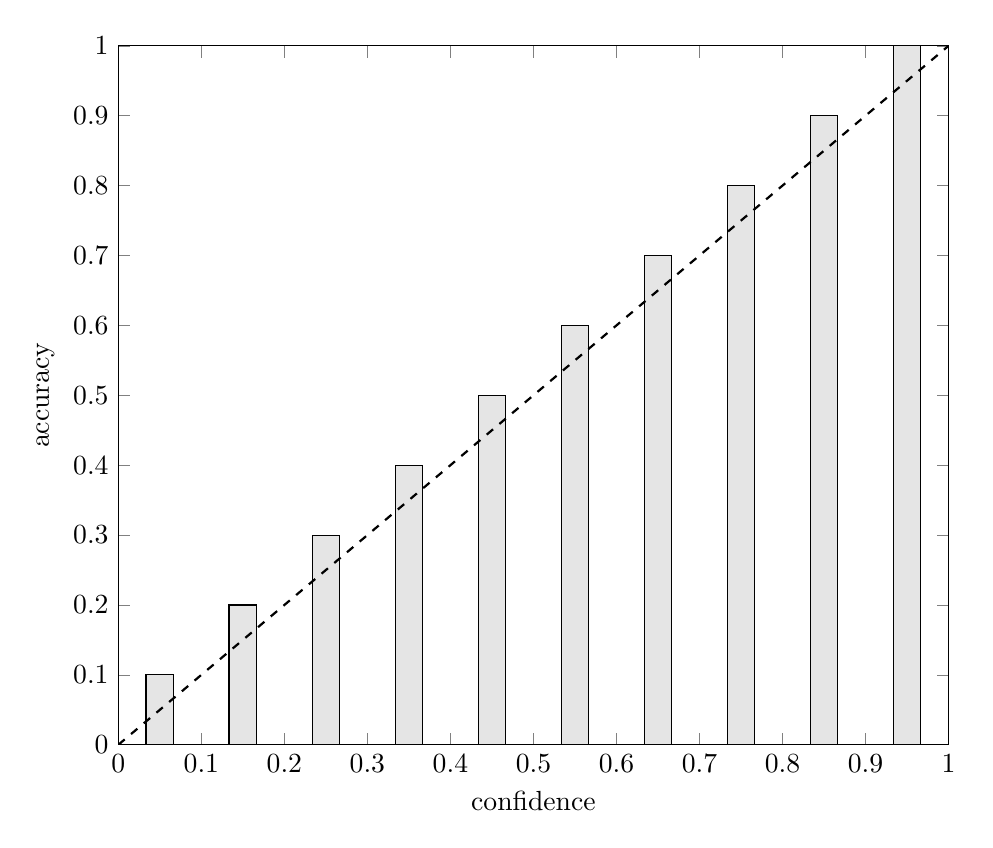
\begin{tikzpicture}
        \begin{axis}[
                width=\textwidth,
                xmin=0,
                xmax=1,
                ymin=0,
                ymax=1,
                xlabel={confidence},
                ylabel={accuracy},
                bar shift=-0.05,
            ]
            \addplot [ybar,fill=black!10] coordinates {
                    (0.1,0.1)
                    (0.2,0.2)
                    (0.3,0.3)
                    (0.4,0.4)
                    (0.5,0.5)
                    (0.6,0.6)
                    (0.7,0.7)
                    (0.8,0.8)
                    (0.9,0.9)
                    (1.0,1.0)
                };
            \addplot [smooth, dashed, thick] coordinates {
                    (0.0,0.0)
                    (1.0,1.0)
                };
        \end{axis}
    \end{tikzpicture}
    \vfill
    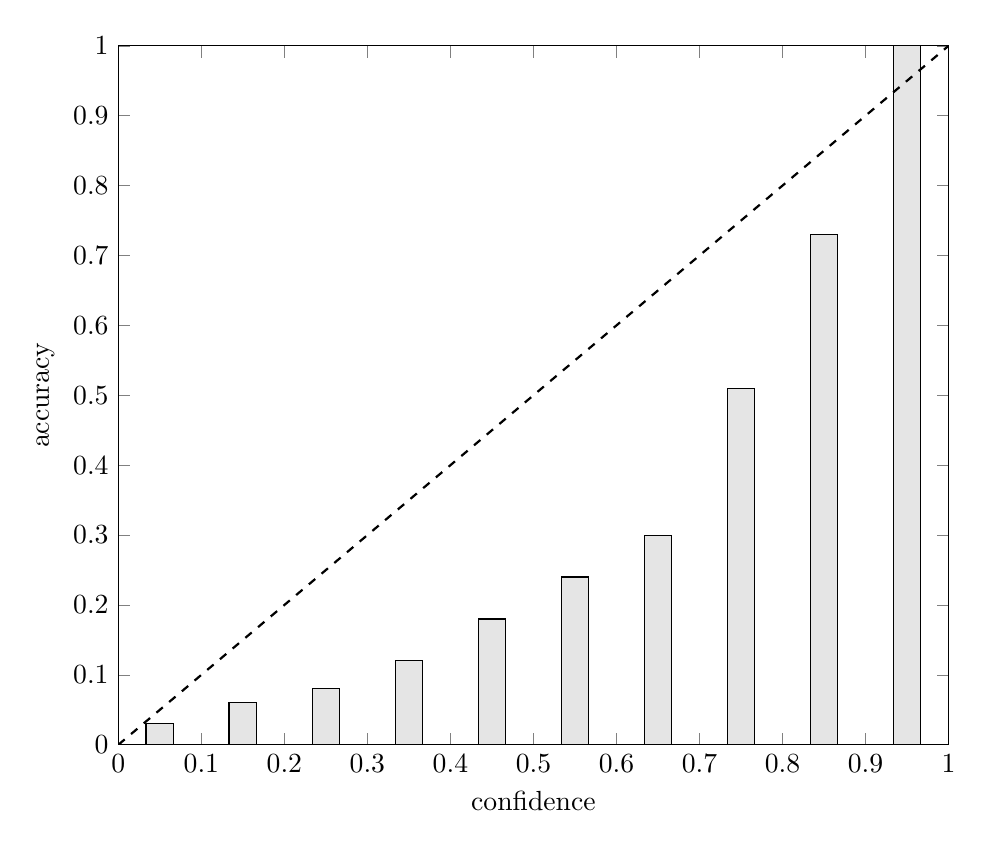
\begin{tikzpicture}
        \begin{axis}[
                width=\textwidth,
                xmin=0,
                xmax=1,
                ymin=0,
                ymax=1,
                xlabel={confidence},
                ylabel={accuracy},
                bar shift=-0.05,
            ]
            \addplot [ybar,fill=black!10] coordinates {
                    (0.1,0.03)
                    (0.2,0.06)
                    (0.3,0.08)
                    (0.4,0.12)
                    (0.5,0.18)
                    (0.6,0.24)
                    (0.7,0.30)
                    (0.8,0.51)
                    (0.9,0.73)
                    (1.0,1.0)
                };
            \addplot [smooth, dashed, thick] coordinates {
                    (0.0,0.0)
                    (1.0,1.0)
                };
        \end{axis}
    \end{tikzpicture}
    \vfill
    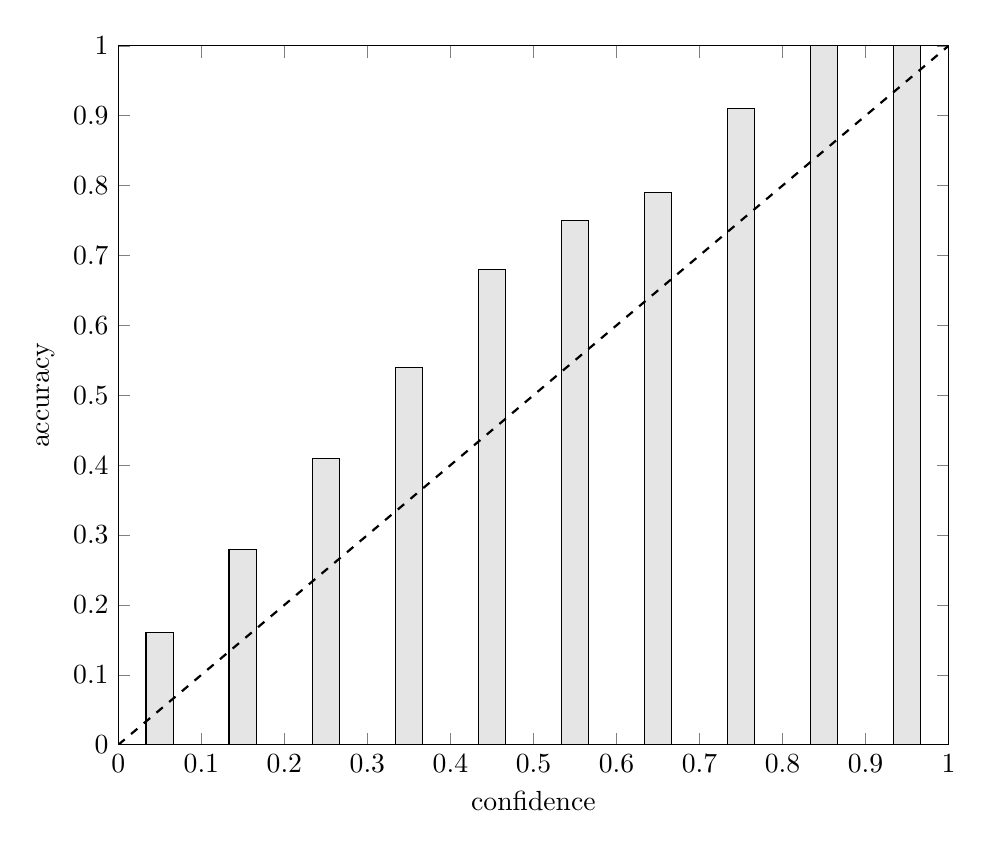
\begin{tikzpicture}
        \begin{axis}[
                width=\textwidth,
                xmin=0,
                xmax=1,
                ymin=0,
                ymax=1,
                xlabel={confidence},
                ylabel={accuracy},
                bar shift=-0.05,
            ]
            \addplot [ybar,fill=black!10] coordinates {
                    (0.1,0.16)
                    (0.2,0.28)
                    (0.3,0.41)
                    (0.4,0.54)
                    (0.5,0.68)
                    (0.6,0.75)
                    (0.7,0.79)
                    (0.8,0.91)
                    (0.9,1.0)
                    (1.0,1.0)
                };
            \addplot [smooth, dashed, thick] coordinates {
                    (0.0,0.0)
                    (1.0,1.0)
                };
        \end{axis}
    \end{tikzpicture}

    \caption{Reliability diagrams. The top diagram shows a well-calibrated model,
        the second diagram is overconfident, and the third diagram is
        underconfident.}
    \label{fig:reliability-diagrams}
\end{marginfigure}

Reliability diagrams (\Cref{fig:reliability-diagrams}) are a way of determining
how calibrated a model is. This diagram is constructed by making predictions on
a validation dataset. These predictions are then divided into $M$ bins
according to the predicted class probability, \[
    B_j = \lft\{ y \; \middle| \; p(y) \in \lft[ \frac{j-1}{m}, \frac{j}{m} \rgt) \rgt\}.
\]
Within each bin, we then compare the predicted probabilities (confidence) with
how often the input actually belonged to the class (frequency),
\begin{align*}
    \mathrm{conf}(B_j) & = \frac{1}{|B_j|} \sum_{y \in B_j} p_{\vec{\theta}}(y)          \\
    \mathrm{acc}(B_j)  & = \frac{1}{|B_j|} \sum_{y \in B_j} \mathbb{1}\{ y = \hat{y} \},
\end{align*}
A model is well-calibrated if $\mathrm{conf}(B_j) \approx \mathrm{acc}(B_j)$
for all bins $B_j$.
